%% For double-blind review submission, w/o CCS and ACM Reference (max submission space)
\documentclass[sigplan,review,anonymous]{acmart}\settopmatter{printfolios=true,printccs=false,printacmref=false}
%% For double-blind review submission, w/ CCS and ACM Reference
%\documentclass[sigplan,review,anonymous]{acmart}\settopmatter{printfolios=true}
%% For single-blind review submission, w/o CCS and ACM Reference (max submission space)
%\documentclass[sigplan,review]{acmart}\settopmatter{printfolios=true,printccs=false,printacmref=false}
%% For single-blind review submission, w/ CCS and ACM Reference
%\documentclass[sigplan,review]{acmart}\settopmatter{printfolios=true}
%% For final camera-ready submission, w/ required CCS and ACM Reference
%\documentclass[sigplan]{acmart}\settopmatter{}


%% Conference information
%% Supplied to authors by publisher for camera-ready submission;
%% use defaults for review submission.
\acmConference[PL'18]{ACM SIGPLAN Conference on Programming Languages}{January 01--03, 2018}{New York, NY, USA}
\acmYear{2018}
\acmISBN{} % \acmISBN{978-x-xxxx-xxxx-x/YY/MM}
\acmDOI{} % \acmDOI{10.1145/nnnnnnn.nnnnnnn}
\startPage{1}

%% Copyright information
%% Supplied to authors (based on authors' rights management selection;
%% see authors.acm.org) by publisher for camera-ready submission;
%% use 'none' for review submission.
\setcopyright{none}
%\setcopyright{acmcopyright}
%\setcopyright{acmlicensed}
%\setcopyright{rightsretained}
%\copyrightyear{2018}           %% If different from \acmYear

%% Bibliography style
\bibliographystyle{ACM-Reference-Format}
%% Citation style
%\citestyle{acmauthoryear}  %% For author/year citations
%\citestyle{acmnumeric}     %% For numeric citations
%\setcitestyle{nosort}      %% With 'acmnumeric', to disable automatic
                            %% sorting of references within a single citation;
                            %% e.g., \cite{Smith99,Carpenter05,Baker12}
                            %% rendered as [14,5,2] rather than [2,5,14].
%\setcitesyle{nocompress}   %% With 'acmnumeric', to disable automatic
                            %% compression of sequential references within a
                            %% single citation;
                            %% e.g., \cite{Baker12,Baker14,Baker16}
                            %% rendered as [2,3,4] rather than [2-4].


%%%%%%%%%%%%%%%%%%%%%%%%%%%%%%%%%%%%%%%%%%%%%%%%%%%%%%%%%%%%%%%%%%%%%%
%% Note: Authors migrating a paper from traditional SIGPLAN
%% proceedings format to PACMPL format must update the
%% '\documentclass' and topmatter commands above; see
%% 'acmart-pacmpl-template.tex'.
%%%%%%%%%%%%%%%%%%%%%%%%%%%%%%%%%%%%%%%%%%%%%%%%%%%%%%%%%%%%%%%%%%%%%%


%% Some recommended packages.
\usepackage{booktabs}   %% For formal tables:
                        %% http://ctan.org/pkg/booktabs
\usepackage{subcaption} %% For complex figures with subfigures/subcaptions
                        %% http://ctan.org/pkg/subcaption


\begin{document}

%% Title information
\title[Short Title]{Virtualization for porting application }         %% [Short Title] is optional;
                                        %% when present, will be used in
                                        %% header instead of Full Title.
%\titlenote{with title note}             %% \titlenote is optional;
                                        %% can be repeated if necessary;
                                        %% contents suppressed with 'anonymous'
\subtitle{or tools to solve a puzzle}                     %% \subtitle is optional
%\subtitlenote{with subtitle note}       %% \subtitlenote is optional;
                                        %% can be repeated if necessary;
                                        %% contents suppressed with 'anonymous'


%% Author information
%% Contents and number of authors suppressed with 'anonymous'.
%% Each author should be introduced by \author, followed by
%% \authornote (optional), \orcid (optional), \affiliation, and
%% \email.
%% An author may have multiple affiliations and/or emails; repeat the
%% appropriate command.
%% Many elements are not rendered, but should be provided for metadata
%% extraction tools.

%% Author with single affiliation.
\author{Théo Rogliano}
\authornote{with author1 note}          %% \authornote is optional;
                                        %% can be repeated if necessary
\orcid{nnnn-nnnn-nnnn-nnnn}             %% \orcid is optional
\affiliation{
  \position{Position1}
  \department{Department1}              %% \department is recommended
  \institution{Institution1}            %% \institution is required
  \streetaddress{Street1 Address1}
  \city{City1}
  \state{State1}
  \postcode{Post-Code1}
  \country{Country1}                    %% \country is recommended
}
\email{first1.last1@inst1.edu}          %% \email is recommended

%% Author with two affiliations and emails.
\author{First2 Last2}
\authornote{with author2 note}          %% \authornote is optional;
                                        %% can be repeated if necessary
\orcid{nnnn-nnnn-nnnn-nnnn}             %% \orcid is optional
\affiliation{
  \position{Position2a}
  \department{Department2a}             %% \department is recommended
  \institution{Institution2a}           %% \institution is required
  \streetaddress{Street2a Address2a}
  \city{City2a}
  \state{State2a}
  \postcode{Post-Code2a}
  \country{Country2a}                   %% \country is recommended
}
\email{first2.last2@inst2a.com}         %% \email is recommended
\affiliation{
  \position{Position2b}
  \department{Department2b}             %% \department is recommended
  \institution{Institution2b}           %% \institution is required
  \streetaddress{Street3b Address2b}
  \city{City2b}
  \state{State2b}
  \postcode{Post-Code2b}
  \country{Country2b}                   %% \country is recommended
}
\email{first2.last2@inst2b.org}         %% \email is recommended


%% Abstract
%% Note: \begin{abstract}...\end{abstract} environment must come
%% before \maketitle command
\begin{abstract}
Migrating applications between language versions is an endeavor task. A developper write an application in a particular version of a language and cannot make preparation to the future language changes. In this article, we explore a solution based on virtualization in the programming language level to port from a version to another. Virtualization is well-known in Operating System (OS). It consists to create a layer with which the application will communicate believing it is the targetted OS. In our case, instead of the OS it is a version of a programming language we target. To do so, we revisit module and virtualization techniques. We chose to validate it by migrating legacy Pharo applications. 
 

\end{abstract}


%% 2012 ACM Computing Classification System (CSS) concepts
%% Generate at 'http://dl.acm.org/ccs/ccs.cfm'.
\begin{CCSXML}
<ccs2012>
<concept>
<concept_id>10011007.10011006.10011008</concept_id>
<concept_desc>Software and its engineering~General programming languages</concept_desc>
<concept_significance>500</concept_significance>
</concept>
<concept>
<concept_id>10003456.10003457.10003521.10003525</concept_id>
<concept_desc>Social and professional topics~History of programming languages</concept_desc>
<concept_significance>300</concept_significance>
</concept>
</ccs2012>
\end{CCSXML}

\ccsdesc[500]{Software and its engineering~General programming languages}
\ccsdesc[300]{Social and professional topics~History of programming languages}
%% End of generated code


%% Keywords
%% comma separated list
\keywords{keyword1, keyword2, keyword3}  %% \keywords are mandatory in final camera-ready submission


%% \maketitle
%% Note: \maketitle command must come after title commands, author
%% commands, abstract environment, Computing Classification System
%% environment and commands, and keywords command.
\maketitle


\section{Introduction}

A software can be view as a patchwork or a puzzle composed by diffrent entities.
	\begin{figure}[H]
       \centering
       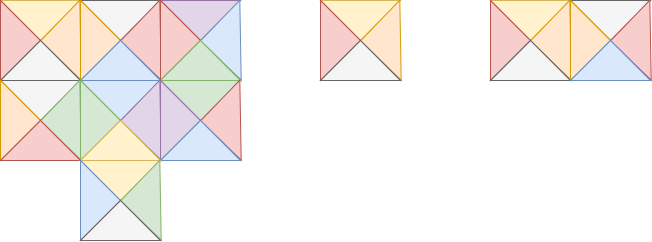
\includegraphics[scale=0.25]{Images/SoftwareAsAPuzzle.png}
           \caption{Left: view of a software as a Puzzle. Middle: a representation of an entity composing a software. Right: representation on a dependancy between two entities.}
	\end{figure}	
These entities and their links are written in a programming langage. However a used langage is an evolving creature.
It means with enough evolution it become impossible to read parts of a software written in an old dialect.
In other words, we lost some pieces of the puzzle.
We identified the following evolutions provoking missing parts:
\begin{description}
    \item[Syntax Changes.] Changes in the syntax make programs that were valid for one version, invalid in another;
    \item[Compiler Semantic Changes.] Changes in the compiler's semantics keep the same syntax as before but change the compiled code's behavior, breaking the code that makes assumptions on it;
    \item[Standard Library Changes.] Changes in the classes of the standard libraries invalidate the code that uses it \textit{e.g.,} methods or classes removed, or methods with modified semantics.
\end{description}
	\begin{figure}[H]
       \centering
       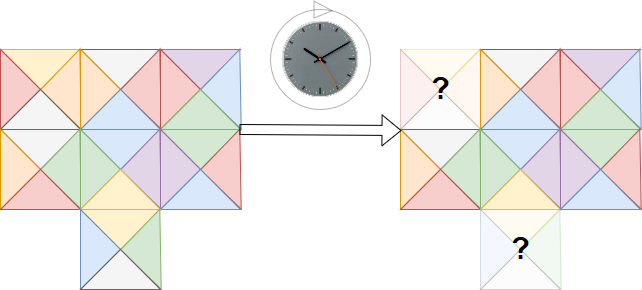
\includegraphics[scale=0.25]{Images/MissingPartAsTimeGoes.png}
        \caption{Missing parts as time goes.}
	\end{figure}
	
One can try to keep the software as much compatible as possible but it is not always possible or straightforward e.g., changes in the language may break the application.

We choose to explore a solution based on virtualization.
Virtualization is well-known in Operating System (OS) and the problem it solve is similar to ours.
OS have differences and a software supported by one OS may not be supported by another due to these differences.
Virtualization is a technique that consist to interpose a layer between a software and an OS.
The role of the layer is: if the behavior is present to transmit calls to the OS else to take care of the calls.
We want to achieve the same results but with programming language instead of OS. 
	\begin{figure}[H]
       \centering
       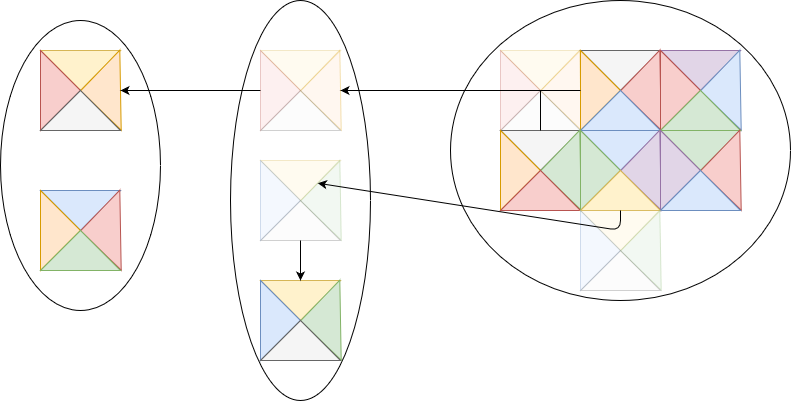
\includegraphics[scale=0.25]{Images/VirtualisationIdea.png}
        \caption{Representation of virtualization technique. The calls to the missing parts are handle by the layer in the middle.}
	\end{figure}
	
In this article, in a first time, we will study the infrastructure needed to construct such a virtualization layer.
In a second time, we will validate the chosen infrastructure with different migrating scenarios of Pharo application.



%% Acknowledgments
\begin{acks}                            %% acks environment is optional
                                        %% contents suppressed with 'anonymous'
  %% Commands \grantsponsor{<sponsorID>}{<name>}{<url>} and
  %% \grantnum[<url>]{<sponsorID>}{<number>} should be used to
  %% acknowledge financial support and will be used by metadata
  %% extraction tools.
  This material is based upon work supported by the
  \grantsponsor{GS100000001}{National Science
    Foundation}{http://dx.doi.org/10.13039/100000001} under Grant
  No.~\grantnum{GS100000001}{nnnnnnn} and Grant
  No.~\grantnum{GS100000001}{mmmmmmm}.  Any opinions, findings, and
  conclusions or recommendations expressed in this material are those
  of the author and do not necessarily reflect the views of the
  National Science Foundation.
\end{acks}


%% Bibliography
%\bibliography{bibfile}
\section{Infrastructure for virtualization}
Through this section, we will details the prerequisites for creating a virtualization layer as we intend (ref fig 3)
The following features are mandatory.

\subsection{Late class creation}
The first hardship is to manage to load our application.
Indeed, the processus of creation of the entities can be the missing part.  
New classes in Pharo are created by evaluating a message \#subclass: send to the superclass.
\begin{verbatim}
    Object subclass: #Car
        instanceVariableNames: 'color name'
        uses: TMovableObject
        classVariableNames: ''
        category:''
\end{verbatim}
The superclass is then in charge of class creation by configuring a class builder with the arguments of the message.
In the case, one of the missing entity is a superclass we cannot create the subclasses.
A similar problem appear with missing trait, the users of the missing trait will not be complete in other words broken. The classes and traits are similar in their creation hence the solution will be the same.

To handle this problem, we kept our classes as a model looking like an Abstract Syntax Tree(AST).
This model is simply a representation of the definition of a class in an easy way.
We enhance the class builder to be configurable with such definition.
We, then, bypass the superclass which allows us to create classes from their definitions.
	\begin{figure}[H]
       \centering
       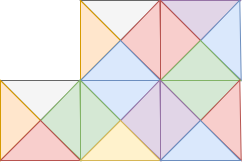
\includegraphics[scale=0.25]{Images/IncompleteSoftware.png}
        \caption{Representation of an incomplete loaded software.}
	\end{figure}

At this point we overlooked the missing pieces, all the non missing parts can almost be loaded but we still need to solve the missing references at least meanwhile we are looking for a better solution.

\subsection{Representation of missing parts}

	\begin{figure}[H]
       \centering
       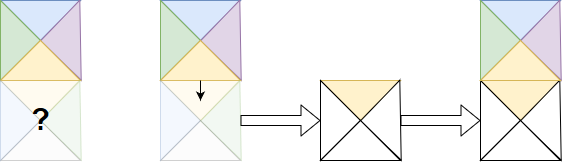
\includegraphics[scale=0.25]{Images/UndefinedExplication.png}
        \caption{The idea behind undefined.}
	\end{figure}
	
	\begin{figure}[H]
       \centering
       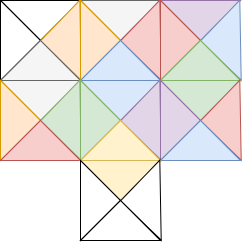
\includegraphics[scale=0.25]{Images/SoftWithUndefined.png}
        \caption{A software with undefined.}
	\end{figure}


\subsection{Encapsulation}
\subsection{Dependancy management}

\section{Validation}

\subsection{Methodology}

\subsection{Results}

\section{Related Work}

\section{Conclusion}

%% Appendix
\appendix
\section{Appendix}

Text of appendix \ldots

\end{document}
